
\section*{Trusted Path}

SGX enclaves provide secure \emph{computation}, as their execution is isolated from other software on the same platform. However, they do not easily lend themselves to secure \emph{user interaction}. The main reason for this is that, in architecture like SGX, enclaves communicate with I/O devices through the untrusted OS. When an enclave needs to receive user input like keyboard presses, it is the responsibility of the OS to pass data from an input device like a keyboard or mouse to the enclave. When an enclave needs to send user output like draw on the screen, it is the responsibility of the OS to forward output data received from the enclave to a user output device like the screen. Such TEE design means that a compromised OS can easily modify any user input and output and read any secrets that are communicated between the user and the enclave. 

User input manipulation can have severe consequences in several application domains and scenarios. For example, if a malicious OS modifies the user input that is provided to a financial enclave, the enclave can be tricked to perform unauthorized payments. If enclaves are used to control safety-critical systems, such as medical devices or industrial systems, user input modifications may cause serious safety and health risks. Also, any enclave that needs to be configured with a password or similar user authentication credential is difficult to implement securely.

The lack of secure user interaction capabilities in the SGX architecture means that enclaves do not support \emph{trusted path} --- a secure channel from the human user to the trusted application. 

%Depending on the application scenario, two different types of trusted paths may be desirable. The first, and more common, the definition of a trusted path is a secure communication channel between the human user and a \emph{local} trusted application like an enclave. The second, and perhaps less common, the definition of the trusted path is one that realizes a secure communication channel between the user and the \emph{remote} server without using any trusted local application in between. 


\subsubsection*{Design Principles}

Several projects have explored the idea of complementing computing platforms with dedicated, trusted hardware for building a trusted path. While proposing extra hardware may be easy, the more difficult and interesting question is what the added hardware should actually do in order to realize a trusted path? To answer this question, we look at noteworthy previous approaches, examine their limitations, and identify general design principles for secure, trusted path implementation.
    
The first well-known approach that we look at is \emph{transaction confirmation}~\cite{filyanov2011uni}. In such a solution, the user first completes the user interaction, such as payment transactions, by interacting with the user interface of the untrusted platform that may be manipulated by an untrusted OS or browser. Once this is done, the user is expected to confirm his input, like a payment value and account number, using a separate hardware token, to detect and prevent any possible input value modifications.

This approach has two main problems. The first is the fact that the user now has to interact with two separate devices and user interfaces, which reduces the usability of the solution. The second, and more severe, the problem is that such extra confirmation step is vulnerable to so-called \emph{user habituation}. Habituation means that user begins, after a few successful transactions, confirming new payments without actually verifying their correctness. These observations lead us to the first design principle.  

\begin{tcolorbox}
\textbf{Principle 1:} Out-of-context security confirmations have a high cognitive load and risk of user habituation. Thus, user interaction should be protected in the context of the normal user interface.
\end{tcolorbox}

The next approach that we examine is \emph{input trace signing}~\cite{IntegriKey}. Here, the main idea is to use a simple hardware device that sits \emph{in-between} a user input device, such as a keyboard, and the untrusted computing platform. The device intercepts and signs every keypress, or similar user input event, and sends a signed trace to the trusted application. (Such technique is also known as ``bump-in-the-wire''~\cite{McCPerRei2006}.) 

Input trace signing meets our first principle because the user does not have to perform additional security checks outside the main UI. However, such solutions are vulnerable to attacks, where the adversary manipulates the user's input by showing false information on the output channel. That is, output manipulation leads to input integrity violation. One example is \emph{fake-typo} attack. Assume that the user types in value ``10'', but the adversary shows ``1'' on the screen. The user is likely to think that he mistyped and press ``0'' again. As a result, a signed trace of ``100'' will be sent to the trusted application. This simple attack leads us to our next design principle.

\begin{tcolorbox}
\textbf{Principle 2:} User input and output integrity cannot be considered in isolation. Both must be protected simultaneously.
\end{tcolorbox}

The last approach that we examine is \emph{secure overlays}. Fidelius~\cite{Fidelius} is an example research system that follows this approach. Fidelius is based on two separate devices. One device intercepts keyboard presses and signs them for the trusted application, while another device intercepts the HDMI output signal and modifies it with secure overlays of security-critical UIs such as payment web forms. 

Fidelius addresses the above-mentioned problems but is still vulnerable to a different type of user input manipulation that we call \emph{early-submission attack}. This attack is possible because Fidelius only protects keyboard input, but not mouse events. While this may seem only a functional limitation, it turns out that it is actually a security problem. Assume again that the intention of the user is to submit value ``10''. Once the user has typed ``1'', the untrusted OS or browser generates a fake mouse event that submits the web form. Given this attack, we can state our last design principle.

\begin{tcolorbox}
\textbf{Principle 3:} All user input modalities must to be protected simultaneously.
\end{tcolorbox}


\subsubsection*{\protection System}

Given these principles, we designed a new trusted path system called \protection. In the following, we focus on the use case where the trusted path is established between the user and a remote web server. That is, we want to protect interactions where the user completes and submits a security-critical web form. The same solution could be easily modified to create a trusted path between the user and a local enclave as well.

Figure~\ref{fig:architecture} shows the overview of \protection system. The central component of the solution is a low-complexity embedded device called \hub that intercepts key presses from a keyboard and movement events from a mouse, tracks mouse movements, and draws secure overlays. 


\begin{figure}[t]
    \begin{center}
        \begin{subfigure}{0.5\textwidth}
        \centering
            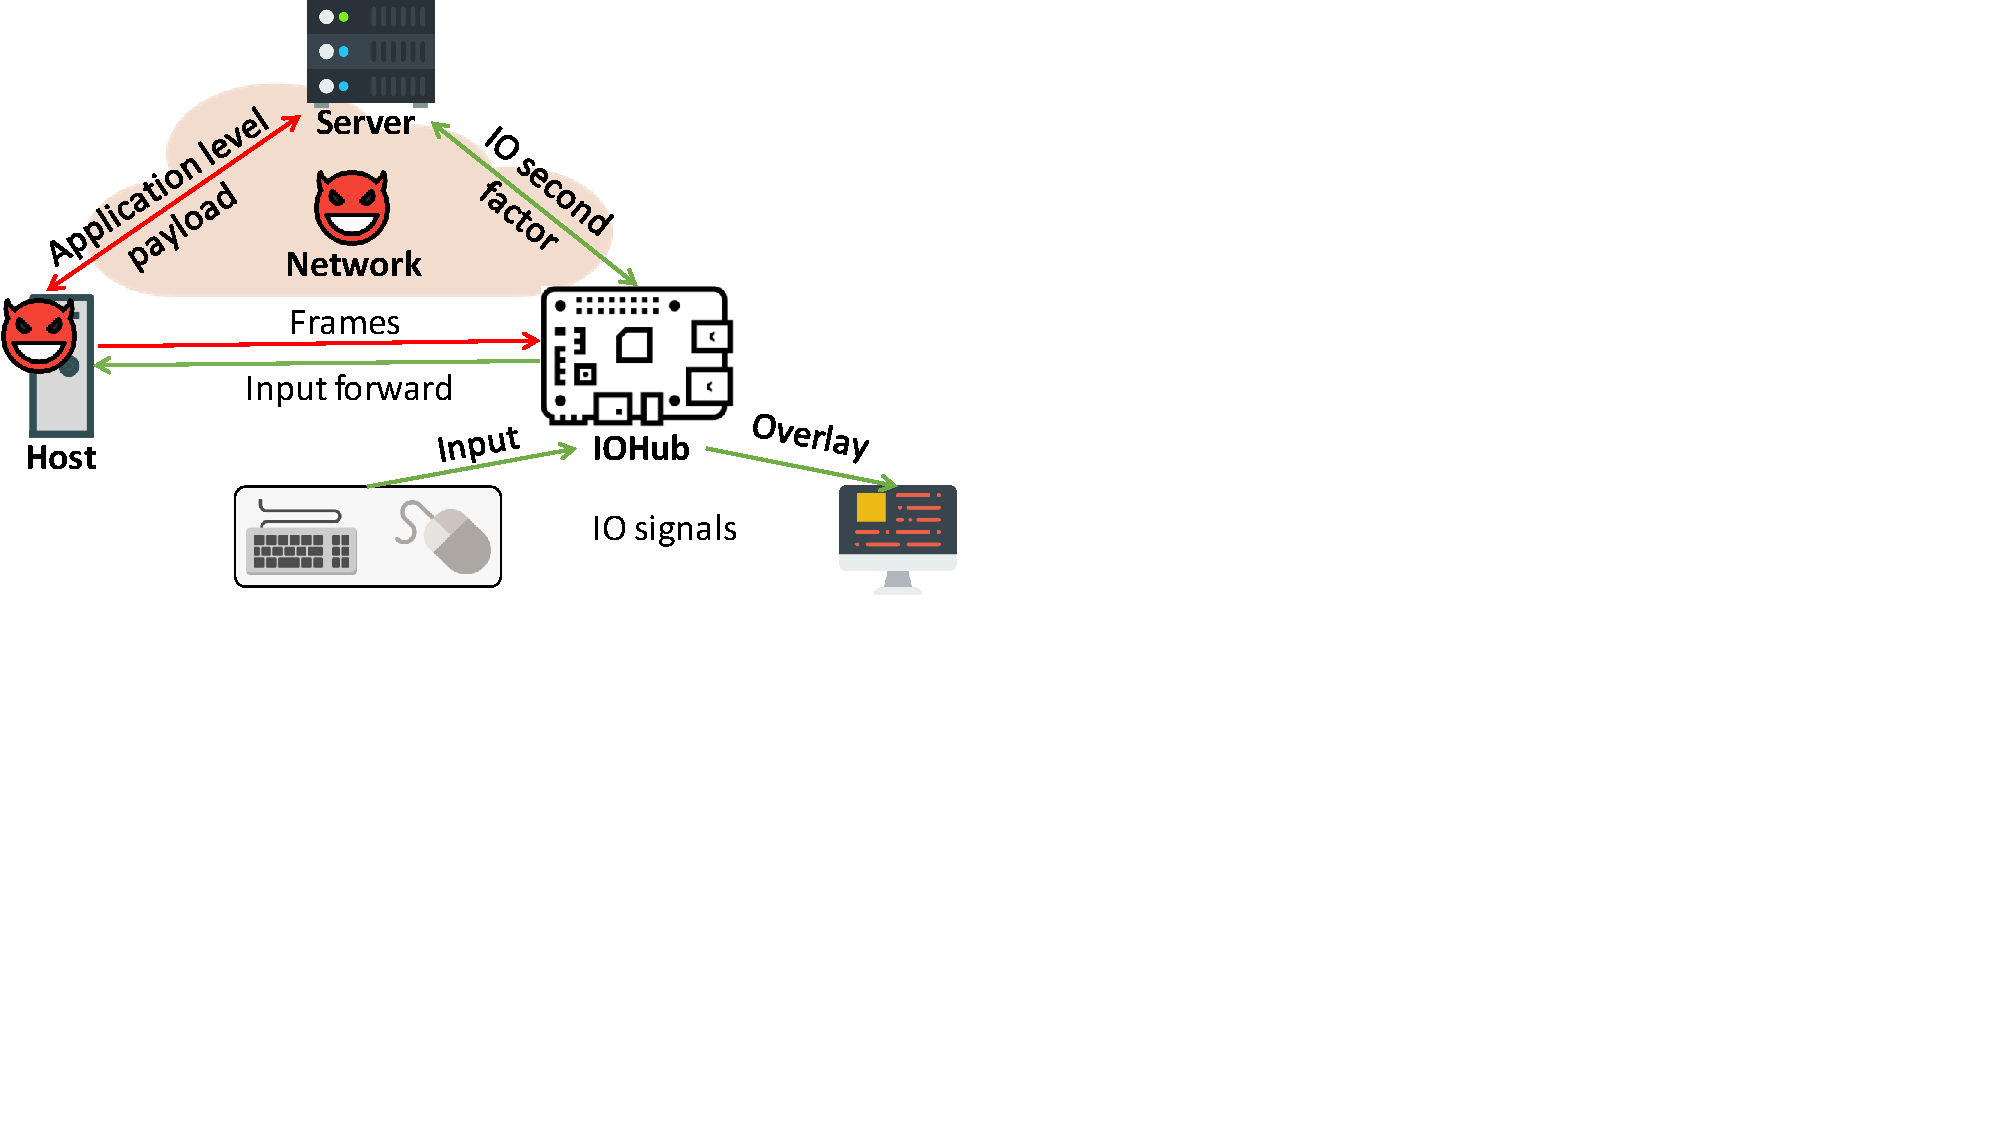
\includegraphics[trim={0 8.5cm 17cm 0}, clip, width=\linewidth]{approachOverview.pdf}
             \caption{\protection system overview.}
            \label{fig:architecture}    
        \end{subfigure}
    \end{center}
    
    %\vspace{1em} 
    
    \begin{center}
        \begin{subfigure}{0.5\textwidth}
        \centering
       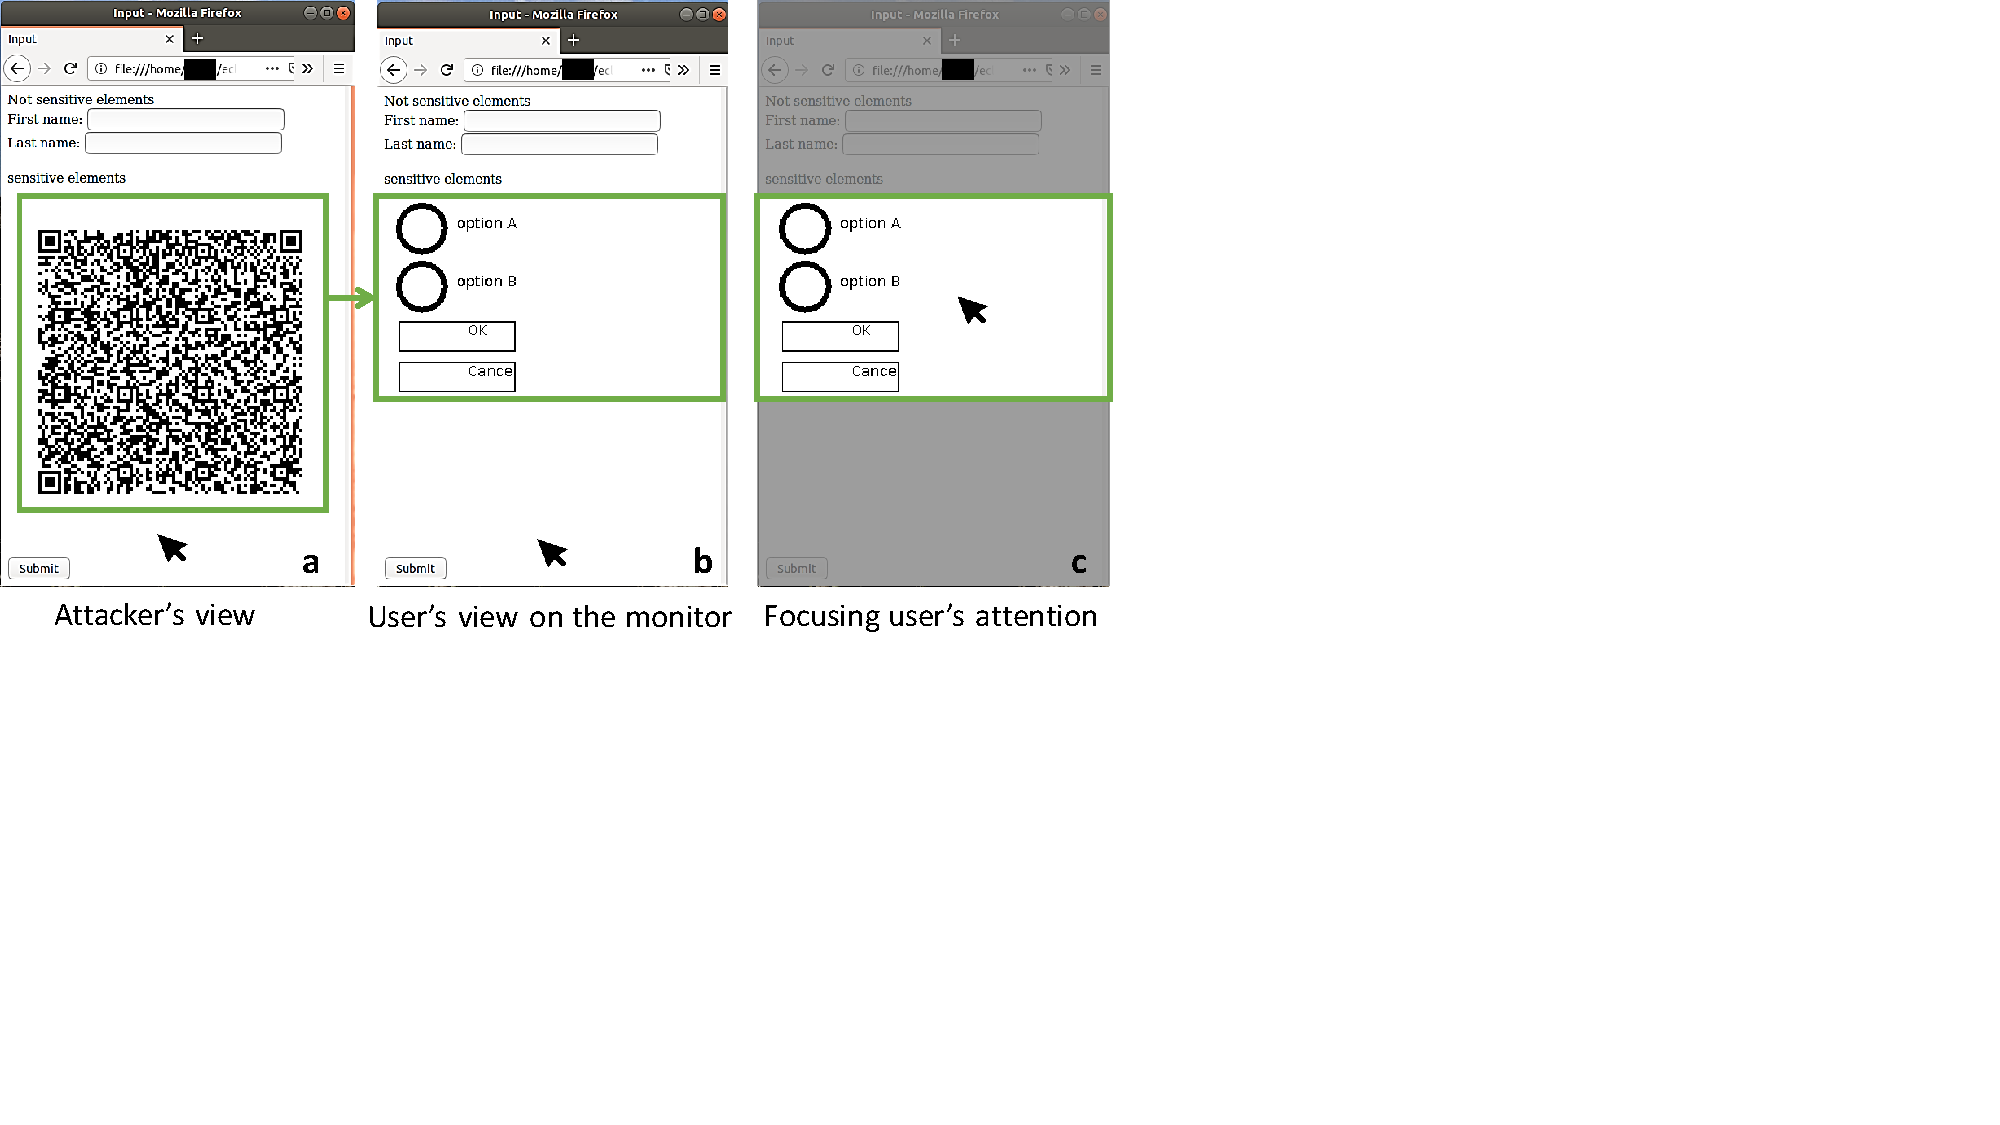
\includegraphics[trim={0 8cm 15cm 0}, clip, width=\linewidth]{overlayScreenShot_new.pdf}
    \caption{\protection user interface. \textbf{(a)} On the left, is shown the view of the attacker, where he sees the QR code that contains the signed UI specification. \textbf{(b)} In the middle, is shown what the user sees after \hub overlays security-sensitive UIs. \textbf{(c)} On the right, is illustrated how \protection focuses user's attention when the user enters the overlaid UI with her mouse.}
        \label{fig:screenshot}
    \end{subfigure}
    \end{center}
    
    \caption{\protection system overview and user interface.} 
    \label{fig:protection}
\end{figure}


% 
% \begin{figure}[t]
%     \centering
%     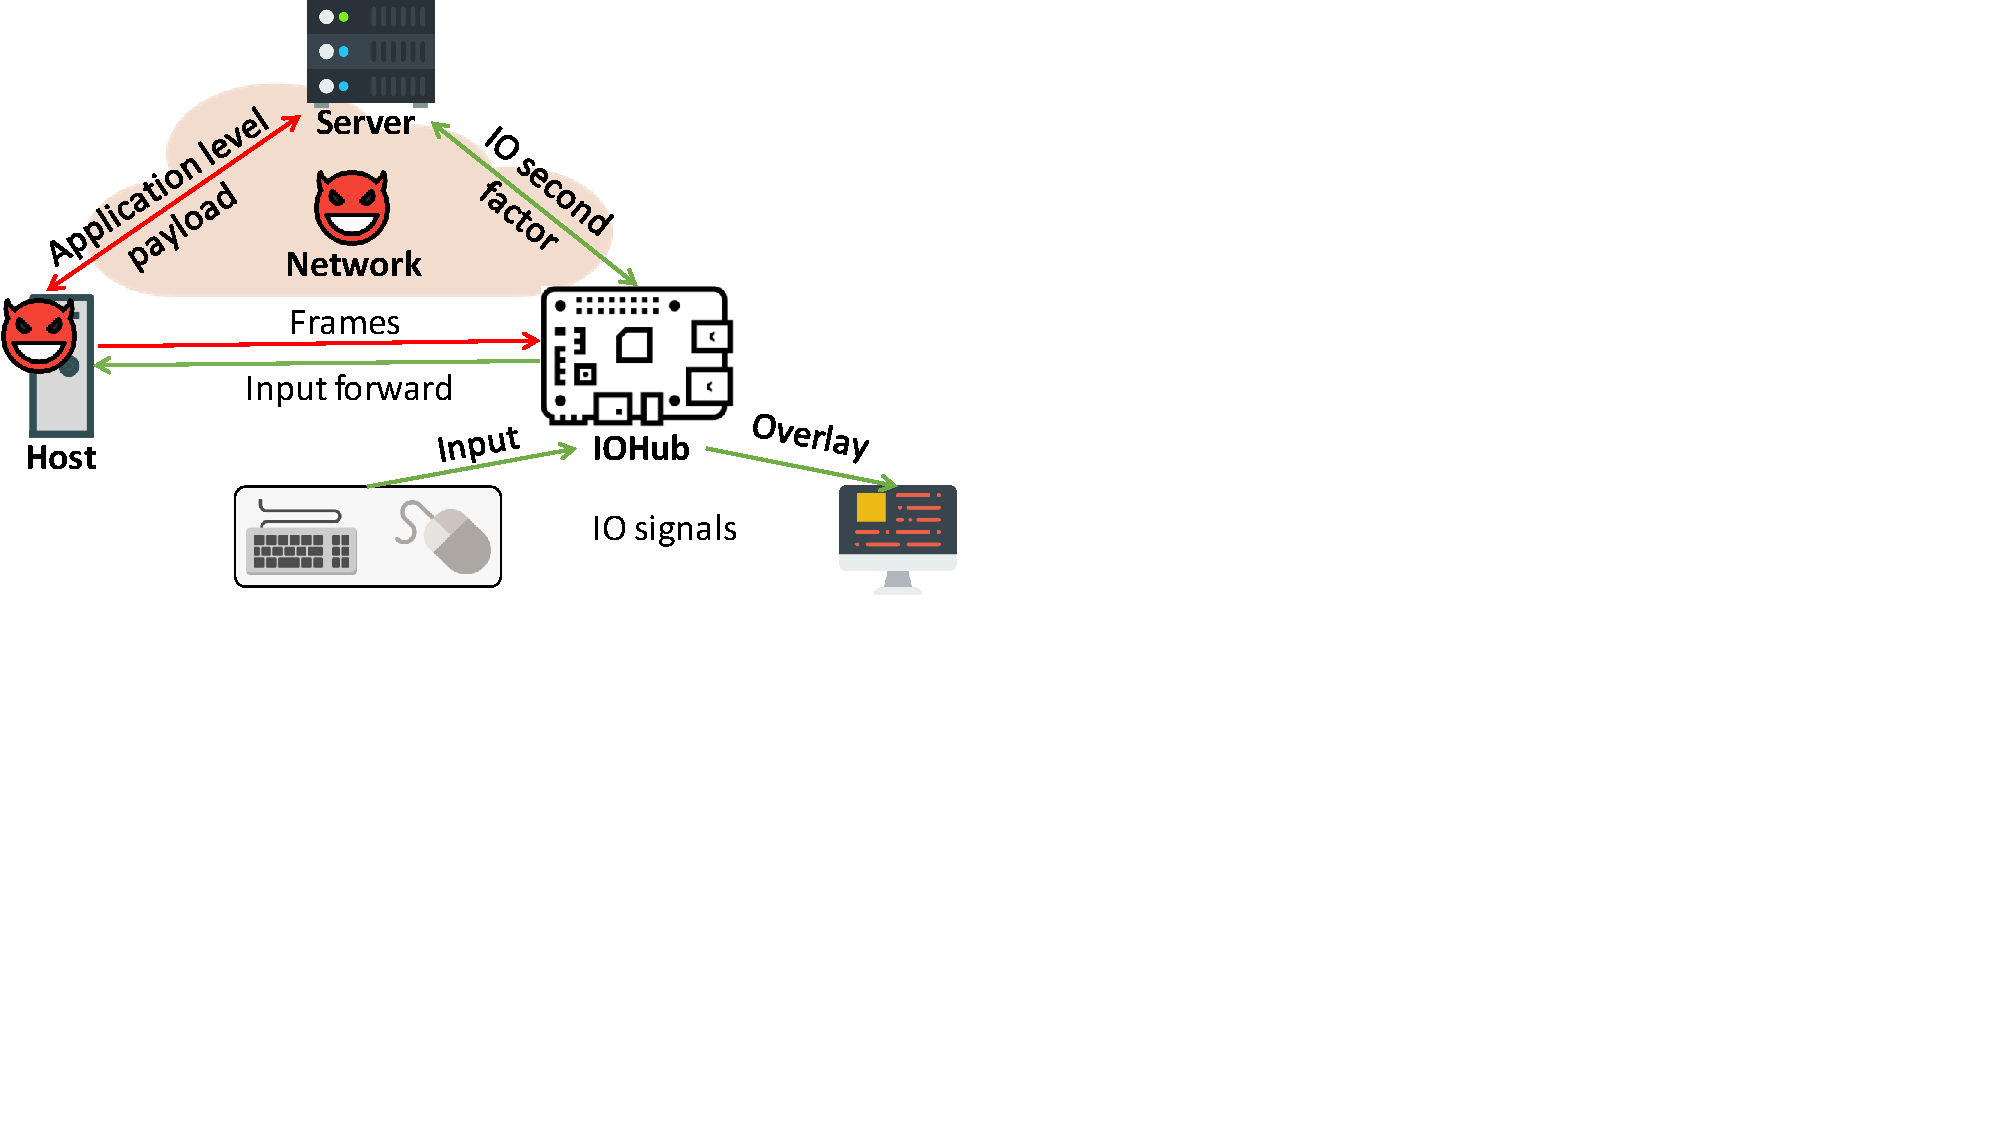
\includegraphics[trim={0 8.5cm 17cm 0}, clip, width=0.9\linewidth]{approachOverview.pdf}
%     \caption{\protection system overview.}
%     \label{fig:architecture}
% \end{figure}
% 
% \begin{figure}[t]
%     \centering
%     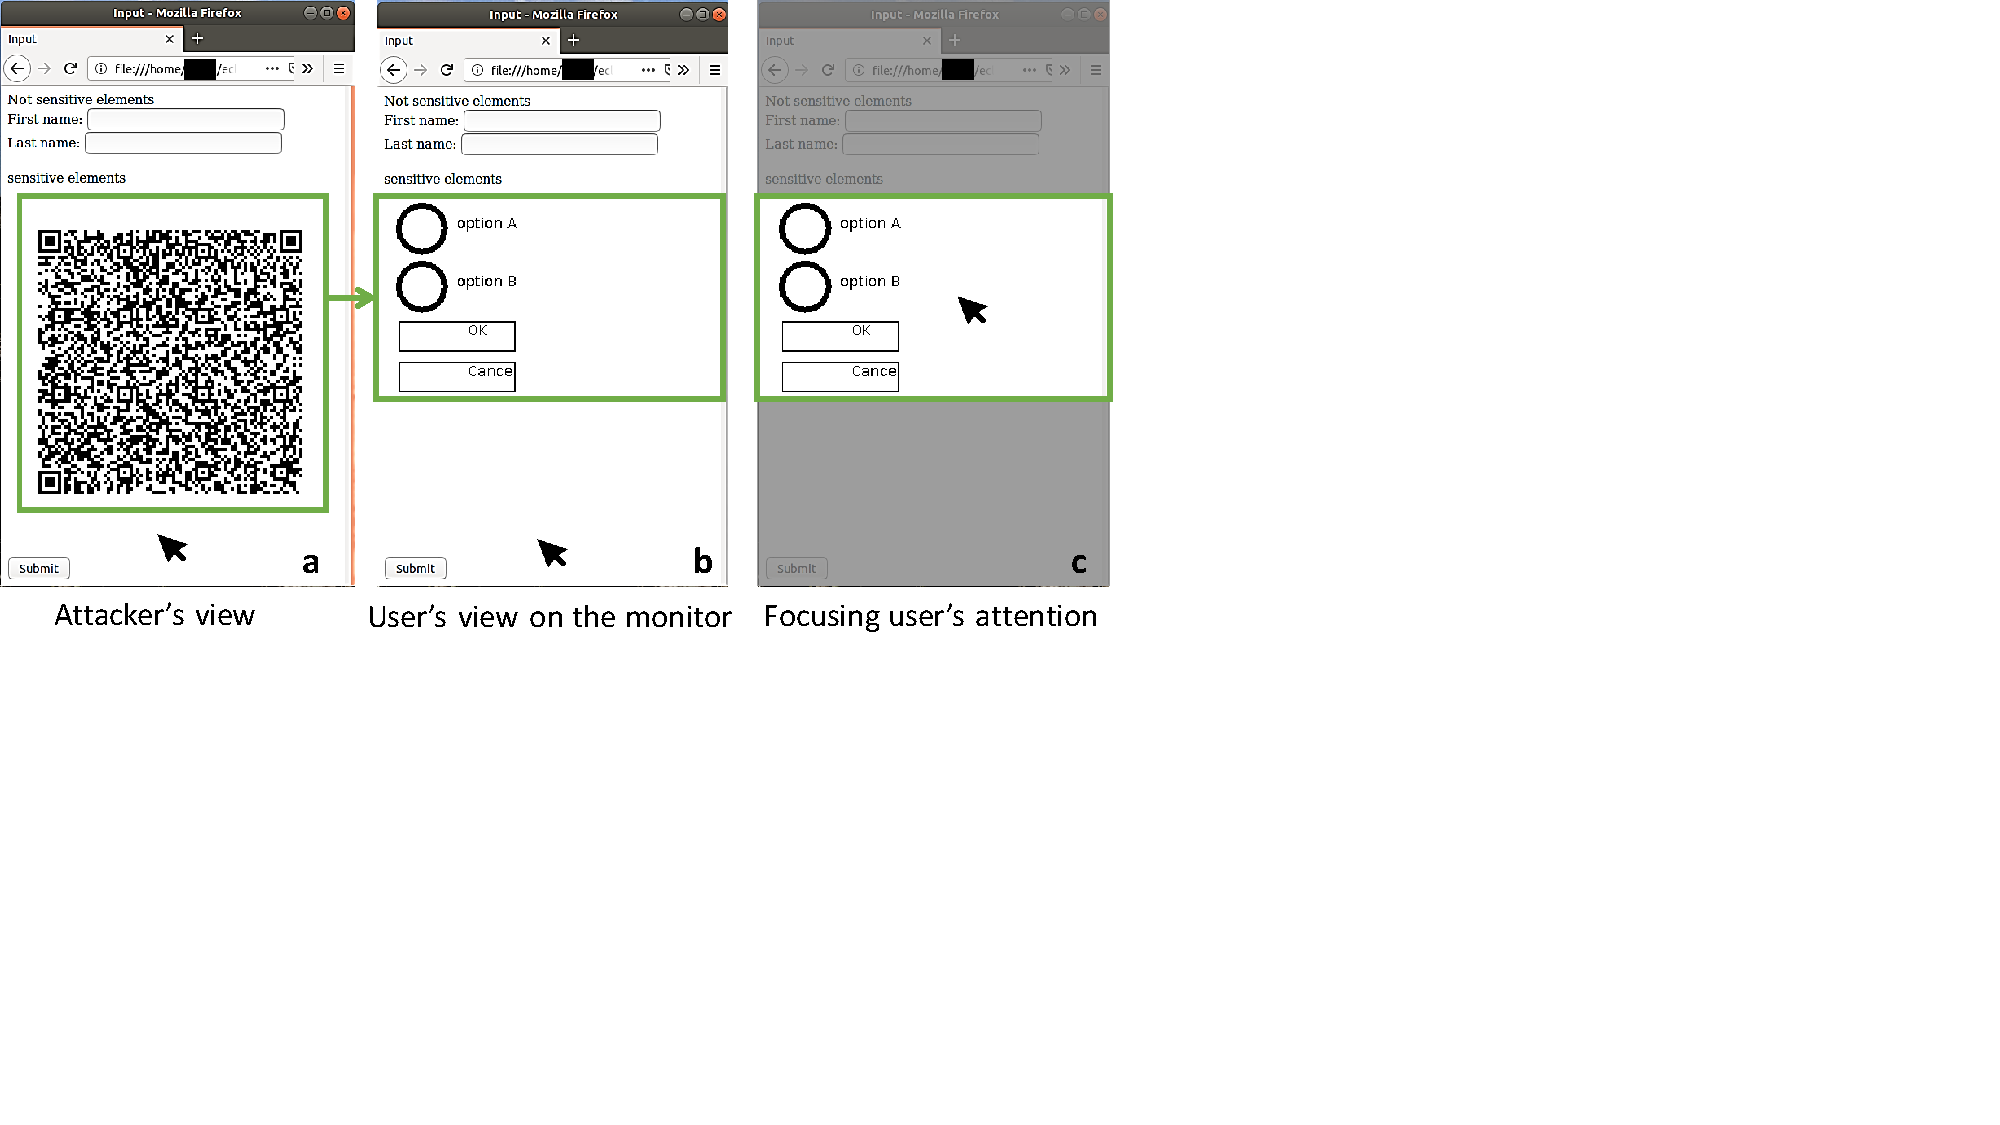
\includegraphics[trim={0 8cm 15cm 0}, clip, width=\linewidth]{overlayScreenShot_new.pdf}
%     \caption{\protection user interface. \textbf{(a)} On the left, is shown the view of the attacker, where he sees the QR code that contains the signed UI specification. \textbf{(b)} In the middle, is shown what the user sees after \hub overlays security-sensitive UIs. \textbf{(c)} On the right, is illustrated how \protection focuses user's attention when the user enters the overlaid UI with her mouse.}
%     \label{fig:screenshot}
% \end{figure}

When the user visits a web page that contains a protected web form, the remote server sends a QR code to the untrusted browser, as shown in Figure~\ref{fig:screenshot} on the left. The QR code contains a specification of the security-critical web form, and the specification is signed by the webserver to prevent its modification by the browser or the OS. By using QR codes, we enable communication from the webserver to the \hub device via an unmodified browser, which simplifies deployment significantly.

By periodically examining the HDMI signal, \hub detects the QR code on the screen, decodes it, and verifies its signature. After that, as is shown in Figure~\ref{fig:screenshot} in the middle, \hub renders the protected web form as an overlay on top of the HDMI frame that it receives from the untrusted OS. This step ensures that the security-critical UI elements are presented to the user as expected, and thus output integrity of the protected web form is preserved.

\hub tracks mouse movement events, and when the mouse pointer enters the secure overlay, as shown in Figure~\ref{fig:screenshot} on the right, \hub dims the rest of the screen to focus the user's attention to the secure overlay. Such protection is needed to prevent the user from following a possible fake mouse cursor drawn by the untrusted browser or OS. Dimming parts of the screen have been shown to be an effective way to focus the user's attention to the correct cursor in the context of clickjacking user studies~\cite{huang2012clickjacking}.

While the user interacts with the protected web form, \hub intercepts all input events, when the user clicks on the submit button, the \hub signs all inputs and sends them to the server via the untrusted browser (e.g., by encoding them to a requested URL). Since the submit button is part of the protected overlay and all mouse clicks are intercepted and signed by the \hub device, early-submission attacks are not possible. The server verifies the signed user inputs it receives. 

If user input confidentiality is needed, the user can be required to trigger a secure attention sequence (SAS), like \texttt{Ctr+Alt+Del}, before entering any secrets. The untrusted OS and the browser cannot observe sensitive data on the secure overlay since they are rendered by \hub and never accessible to them.

\protection complies with our three design principles. Principle 1 is met, as the user only interacts with the main UI. Secure overlays support Principle 2, and mouse tracking combined with input trace signing ensures that all input modalities are protected (Principle 3).

% \begin{figure}[t]
%     \centering
%     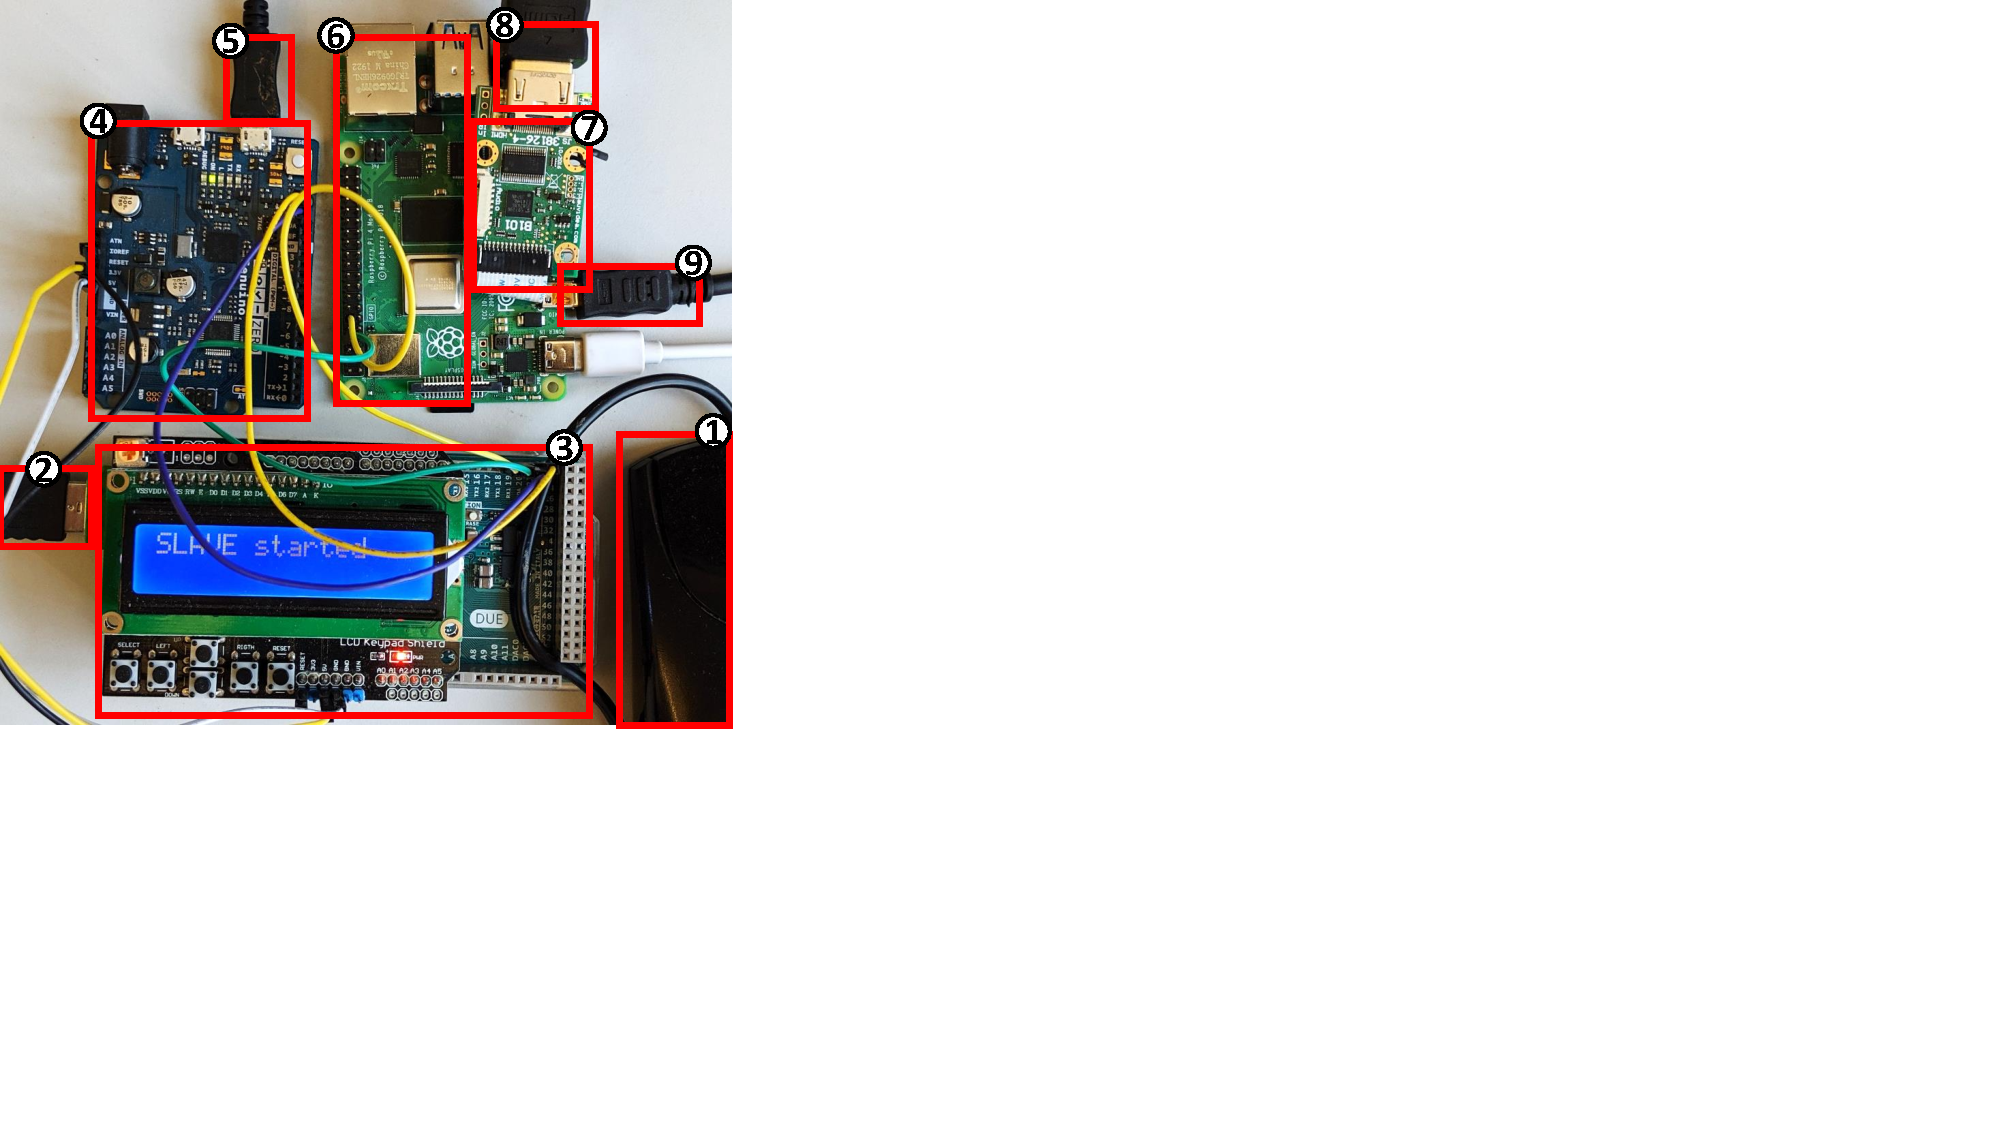
\includegraphics[trim={0 6.6cm 21.5cm 0}, clip, scale=0.5]{setUp_1.pdf}
%     \caption{\protection prototype.}
% \label{fig:prototype}   
% \end{figure}

%\paragraph{Prototype} 
We implemented a prototype of \protection that includes a Raspberry Pi board as a computing unit, an Arduino board as a keyboard and mouse event input interceptor, and a separate HDMI interceptor board. Such a prototype shows that proposed functionalities are feasible to implement on low-cost hardware. Full details of the \protection system are explained in~\cite{protection}.

%The delay in forwarding keystrokes is $170\ \mu s$ and for frames is $21.76\ ms$. This allows the \protection to achieve the maximum display frame rate of $47.69$ per second (e.g., most of the movies are shot and shown in  ~24-30 fps).
